\chapter{Revisão Bibliográfica}

O processamento de imagens é uma ferramenta essencial para garantir a confiabilidade do Sistema Elétrico de Potência (SEP), especialmente na detecção e classificação de falhas em equipamentos de linhas de transmissão de energia elétrica. Essa técnica permite identificar problemas em componentes como isoladores, fixadores e suportes, que, se não tratados, podem causar interrupções no fornecimento de energia. O uso de imagens capturadas por drones ou câmeras especiais facilita a inspeção de grandes extensões de linhas de transmissão, reduzindo custos e aumentando a segurança ao evitar a necessidade de intervenções manuais em locais de difícil acesso \cite{eze2022deep}.

Métodos avançados de análise de imagens, como os baseados em aprendizado profundo, ajudam a reconhecer padrões que indicam falhas, mesmo em condições adversas, como baixa visibilidade ou equipamentos desgastados \cite{Altaie2023}. Essas abordagens são particularmente úteis em regiões com infraestrutura antiga, onde a manutenção regular é desafiadora. Além disso, o processamento de imagens possibilita uma resposta rápida a problemas, minimizando o impacto de falhas na rede elétrica e melhorando a continuidade do serviço \cite{kumar2023novel}.

A automação proporcionada pelo processamento de imagens também contribui para a eficiência operacional. Técnicas modernas permitem monitorar equipamentos em tempo real, identificando danos antes que se tornem críticos \cite{eze2022deep}. Isso é crucial para manter a estabilidade do SEP, especialmente em áreas remotas ou com alta demanda energética. Assim, o processamento de imagens não apenas aprimora a manutenção das linhas de transmissão, mas também reforça a segurança e a confiabilidade do fornecimento de energia elétrica.

A seguir, será apresentada uma revisão dos principais conceitos e técnicas de processamento de imagens, que podem ser aplicados na detecção e classificação de falhas em equipamentos de linhas de transmissão de energia elétrica.

\section{Processamento de Imagens}

O processamento de imagens desempenha um papel fundamental no contexto do Sistema Elétrico de Potência (SEP), especialmente em atividades de inspeção, manutenção preditiva e monitoramento de ativos em linhas de transmissão. Com o uso crescente de drones, câmeras térmicas e sensores ópticos, a obtenção de imagens de componentes da rede elétrica tornou-se mais acessível e eficiente. No entanto, a qualidade e a variabilidade dessas imagens exigem técnicas robustas de pré-processamento para garantir resultados precisos em tarefas como a detecção de falhas, corrosões, aquecimentos anômalos e objetos estranhos nas estruturas. Esta seção apresenta os principais métodos de processamento de imagens empregados para preparar dados visuais que serão utilizados em modelos baseados em aprendizado de máquina e redes neurais, contribuindo diretamente para a confiabilidade, segurança e eficiência operacional do SEP.

\subsection{Normalização}
A normalização é uma etapa fundamental no pré-processamento de imagens para redes neurais, pois padroniza os valores dos pixels, facilitando a convergência durante o treinamento e melhorando a generalização do modelo. Um método comum é a normalização de valores de pixels, que escala os valores para intervalos como [0,1] ou [-1,1], frequentemente realizada dividindo os valores originais pelo máximo possível (por exemplo, 255 para imagens de 8 bits) \cite{sharma2024deep}. Outro método é a normalização Z-score, que subtrai a média dos pixels e divide pelo desvio padrão, resultando em dados com média zero e variância unitária \cite{chen2023robustness}. A equalização de histograma também é utilizada para redistribuir as intensidades dos pixels, aumentando o contraste e destacando detalhes em imagens de baixa qualidade \cite{chen2023robustness}. Além disso, a padronização de cores, como subtrair os valores médios dos canais RGB, centraliza os dados em torno de uma distribuição normal, o que é particularmente útil para redes convolucionais \cite{sciencedirect2023normalization}. Técnicas mais avançadas, como a normalização por percentis, utilizam o 5º e o 95º percentis como limites para lidar com valores discrepantes, enquanto a correspondência de histogramas ajusta a distribuição de intensidades com base em pontos de referência \cite{isola2023comparison}. Essas abordagens garantem que as redes neurais processem dados de forma consistente, reduzindo a sensibilidade a variações de iluminação ou escala, especialmente em tarefas de visão computacional \cite{sharma2024deep}.

A Figura \ref{fig:normalizacao} ilustra o processo de normalização de imagens, onde a imagem original é transformada em uma imagem normalizada, facilitando a extração de características relevantes.

\begin{figure}[H]
    \centering
    \caption{\label{fig:normalizacao}Normalização de Imagens}
    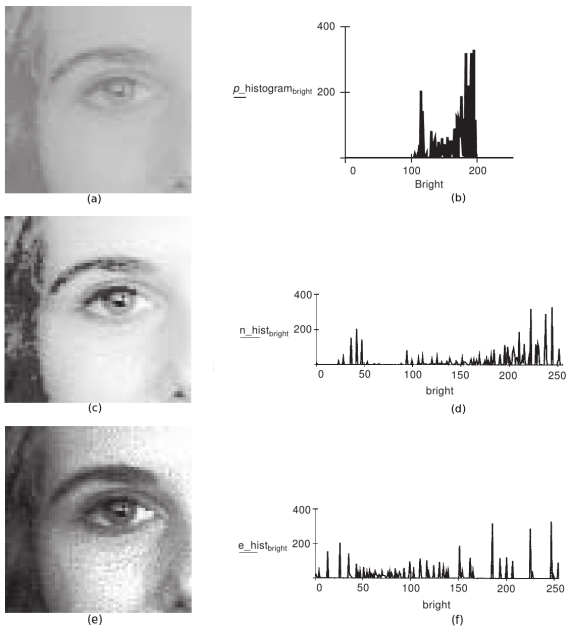
\includegraphics[width=0.8\textwidth]{img/revisao_bibliografica/normalizacao.png}
    \fonte{\citeonline{kuehlkamp2013ferramenta}.}
\end{figure}

\subsection{Redimensionamento e Recorte}
O redimensionamento é essencial para ajustar as imagens ao tamanho de entrada esperado pelas arquiteturas de redes neurais, garantindo compatibilidade e consistência. Um método comum é redimensionar as imagens para um tamanho fixo, como 224x224 pixels, amplamente utilizado em modelos como ResNet e VGG \cite{chen2023robustness}. Isso pode ser feito por meio de interpolação bilinear ou bicúbica, que suaviza as transições entre pixels, embora métodos mais avançados, como interpolação baseada em Fourier, também sejam explorados \cite{dennanni2019resizing}. O recorte, por outro lado, extrai uma região de interesse da imagem, frequentemente centrada, para preservar áreas relevantes, especialmente quando as dimensões originais variam significativamente \cite{sciencedirect2023normalization}. Estudos indicam que o redimensionamento para tamanhos menores pode acelerar o treinamento, mas tamanhos muito reduzidos podem comprometer a qualidade das características extraídas \cite{sabottke2020effect}. Além disso, o recorte aleatório é usado em conjunto com aumento de dados para introduzir variabilidade durante o treinamento \cite{nalepa2022data}. Essas técnicas são cruciais para lidar com conjuntos de dados heterogêneos, garantindo que as entradas sejam uniformes sem perda significativa de informação \cite{chen2023robustness}.

A Figura \ref{fig:redimensionamento_e_recorte} ilustra o processo de redimensionamento e recorte de imagens, na qual a imagem da esquerda (original) é utilizada para extrair uma região de interesse (recorte) e em seguida redimensionada para um tamanho fixo (imagem da direita).

\begin{figure}[H]
    \centering
    \caption{\label{fig:redimensionamento_e_recorte}Redimensionamento e recorte}
    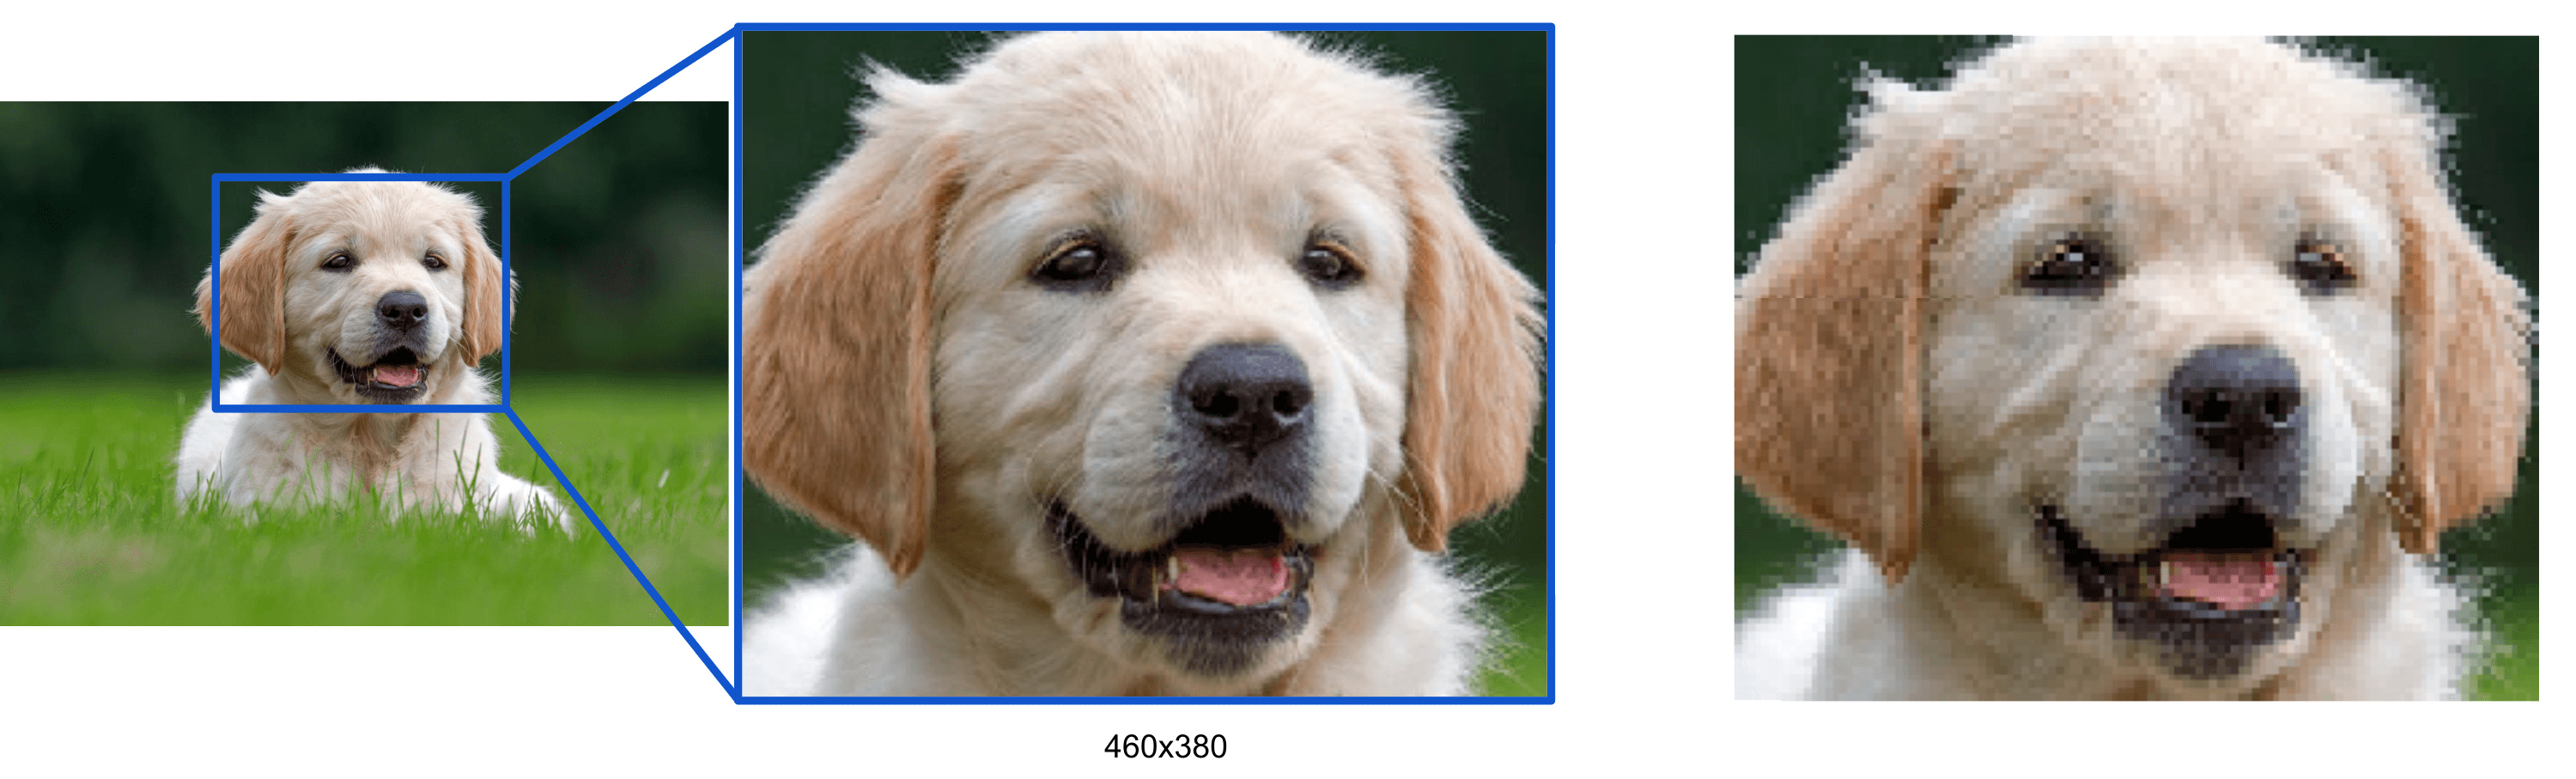
\includegraphics[width=1\textwidth]{img/revisao_bibliografica/redimensionamento_e_recorte.png}
    \fonte{Adaptado de \citeonline{venturelli2021}.}
\end{figure}

\subsection{Aumento de Dados}
O aumento de dados é uma estratégia poderosa para ampliar a diversidade do conjunto de treinamento, reduzindo o risco de sobreajuste e melhorando a robustez do modelo. Técnicas geométricas incluem espelhamento horizontal ou vertical, rotações em ângulos variados (de 1° a 359°), translações, cortes aleatórios e ajustes de escala, que simulam diferentes perspectivas e tamanhos \cite{shorten2019survey}. Transformações no espaço de cores, como ajustes de brilho, contraste, saturação e matiz, ajudam a lidar com variações de iluminação \cite{shorten2019survey}. Métodos mais avançados, como apagamento aleatório, mascaram partes da imagem para simular oclusões, enquanto a mistura de imagens combina pixels de diferentes amostras para criar novas instâncias \cite{shorten2019survey}. Por exemplo, o método SamplePairing reduziu o erro no conjunto CIFAR-10 de 8,22\% para 6,93\% \cite{shorten2019survey}. Além disso, redes adversárias generativas (GANs) são usadas para gerar imagens sintéticas, especialmente em domínios com dados limitados, como imagens médicas, alcançando melhorias de até 10\% em precisão \cite{shorten2019survey}. Essas técnicas são particularmente valiosas em cenários com poucos dados, permitindo que as redes neurais generalizem melhor para condições não vistas \cite{nalepa2022data}.

\subsection{Redução de Ruído}
A redução de ruído remove interferências que podem comprometer o desempenho das redes neurais, sendo especialmente crítica em aplicações como imagens médicas e vigilância. Métodos tradicionais, como filtros de média ou mediana, são complementados por abordagens baseadas em aprendizado profundo, como redes neurais convolucionais (CNNs) especializadas, como DnCNNs, que aprendem a mapear imagens ruidosas para versões limpas \cite{sharma2024deep}. Autoencoders também são empregados para reconstruir imagens a partir de representações latentes, eliminando ruídos como Gaussianos ou de sal e pimenta \cite{sharma2024deep}. Técnicas como Total Variation Denoising (TVD) e Non-Local Means (NLM) exploram regularizações e similaridades entre pixels para preservar detalhes \cite{sharma2024deep}. Um estudo demonstrou que a aplicação de DnCNNs em imagens de tomografia computadorizada resultou em uma precisão de detecção de câncer de pulmão variando de 86,17\% a 99,67\% \cite{sharma2024deep}. Além disso, métodos baseados em redes neurais profundas, como o Deep Neural Filter (DNF), alcançaram melhorias de até 10 dB na relação sinal-ruído em sinais de EEG \cite{peer2022real}. Essas abordagens são essenciais para garantir que as redes neurais processem imagens de alta qualidade, minimizando artefatos que poderiam obscurecer características críticas \cite{sharma2024deep}.

A Figura \ref{fig:reducao_de_ruido} ilustra o processo de redução de ruído, onde a imagem original (à esquerda) é processada para remover o ruído, resultando em uma imagem mais limpa (à direita).

\begin{figure}[H]
    \centering
    \caption{\label{fig:reducao_de_ruido}Redução de Ruído}
    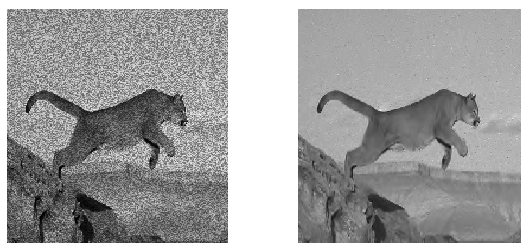
\includegraphics[width=1\textwidth]{img/revisao_bibliografica/reducao_de_ruido.png}
    \fonte{Adaptado de \citeonline{wavelet_denoising}.}
\end{figure}

\subsection{Ajuste de Contraste e Brilho}
O ajuste de contraste e brilho melhora a visibilidade das características das imagens, sendo crucial para tarefas que dependem de detalhes finos. A equalização de histograma redistribui as intensidades dos pixels para maximizar o contraste, enquanto a equalização adaptativa limitada por contraste (CLAHE) evita a amplificação excessiva de ruído em regiões homogêneas \cite{sciencedirect2023normalization}. A correção gama ajusta a curva de intensidade para realçar detalhes em áreas escuras ou claras, sendo amplamente usada em imagens de baixa qualidade \cite{sciencedirect2023normalization}. Métodos baseados em aprendizado profundo, como redes convolucionais fuzzy, integraram filtros Gaussianos e triangulares para melhorar imagens de íris, alcançando até 97\% de precisão em tarefas de reconhecimento \cite{sharma2024deep}. Além disso, técnicas como RetinexDIP foram propostas para melhorar a resolução e reduzir o consumo de memória em comparação com métodos tradicionais \cite{sharma2024deep}. Essas abordagens são fundamentais para preparar imagens para redes neurais, garantindo que as características relevantes sejam destacadas \cite{sciencedirect2023normalization}.

% imagem de exemplo do CLAHE. cite isso no texto abaixo
A Figura \ref{fig:clahe} ilustra o efeito do CLAHE em uma imagem, destacando detalhes que antes estavam obscurecidos.

\begin{figure}[H]
    \centering
    \caption{\label{fig:clahe}Ajuste de Contraste e Brilho com CLAHE}
    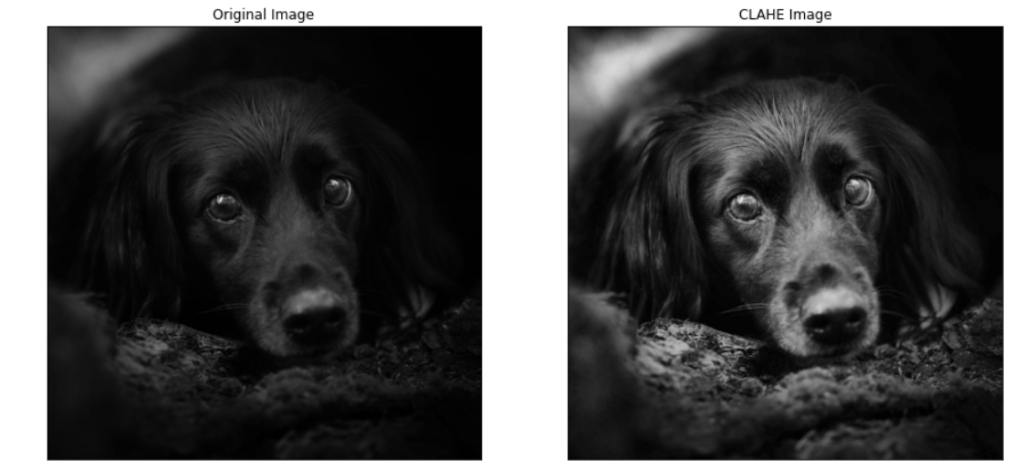
\includegraphics[width=1\textwidth]{img/revisao_bibliografica/clahe.png}
    \fonte{\citeonline{pandey2023image}.}
\end{figure}

\subsection{Aumento de Nitidez}
O aumento de nitidez realça bordas e detalhes finos, facilitando tarefas como detecção de objetos e segmentação. Técnicas tradicionais, como a máscara de desfoque, aplicam filtros de alta passagem para enfatizar transições de intensidade \cite{sciencedirect2023normalization}. Métodos baseados em redes neurais, como CNNs, foram desenvolvidos para detectar e corrigir nitidez, como no caso da detecção de máscaras de desfoque (USM), superando métodos baseados em codificação ternária perpendicular a bordas \cite{ding2018detecting}. Em aplicações específicas, como imagens de documentos, redes convolucionais combinadas com filtros de Gabor e desfoque melhoraram a legibilidade, reduzindo distorções como sombras e ruídos \cite{ben2022deep}. Essas técnicas são particularmente úteis em cenários onde a clareza das bordas é essencial para o desempenho do modelo \cite{sharma2024deep}.

A Figura \ref{fig:aumento_de_nitidez} ilustra o efeito do aumento de nitidez em uma imagem, onde os detalhes são mais evidentes após o processamento.

\begin{figure}[H]
    \centering
    \caption{\label{fig:aumento_de_nitidez}Aumento de Nitidez}
    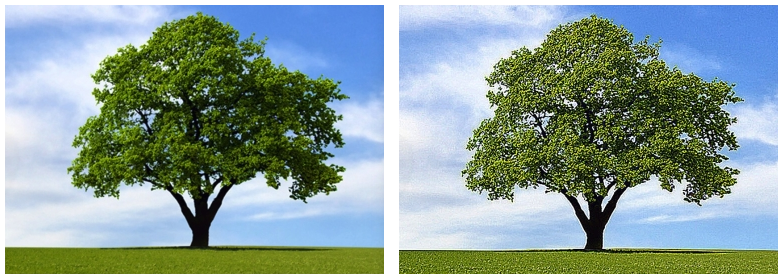
\includegraphics[width=1\textwidth]{img/revisao_bibliografica/aumento_de_nitidez.png}
    \fonte{Adaptado de \citeonline{joshi2025}.}
\end{figure}

\subsection{Conversão de Espaço de Cores}
A conversão de espaço de cores adapta as imagens às necessidades específicas da tarefa, simplificando o processamento ou destacando características relevantes. A conversão de RGB para escala de cinza reduz a dimensionalidade, sendo útil em tarefas onde a cor não é essencial \cite{sharma2024deep}. Espaços como HSV e LAB são preferidos em aplicações que requerem separação de matiz, saturação ou luminância, como segmentação de objetos \cite{sharma2024deep}. Redes neurais também foram usadas para realizar conversões de espaço de cores, como de RGB para XYZ, alcançando erros de cor inferiores a 1,0 unidade ΔE 2000 em mais de 85\% dos casos testados \cite{macdonald2019color}. Essas conversões são valiosas para otimizar a extração de características e reduzir a complexidade computacional em tarefas de visão computacional \cite{sharma2024deep}.

\subsection{Restauração e Desembaçamento de Imagens}
A restauração de imagens visa recuperar a imagem original a partir de versões degradadas por desfoque, ruído ou outras distorções. O desembaçamento, um subcampo da restauração, utiliza redes neurais como U-Net para corrigir desfoques dinâmicos, alcançando PSNR de 31,53 no conjunto GoPro e 31,32 no Real Blur \cite{Lian2023Deblurring}. Métodos baseados em autoencoders convolucionais foram propostos para restaurar imagens em aplicações de fotografia computacional e sensoriamento remoto \cite{barreto2020cnn}. Além disso, redes neurais como DnCNNs foram aplicadas para remover ruídos específicos, como speckle em imagens holográficas \cite{sharma2024deep}. Essas técnicas são cruciais para preparar imagens de alta qualidade para redes neurais, especialmente em domínios onde a clareza é essencial \cite{sumida2019deep}.

A Figura \ref{fig:desembacamento} ilustra o processo de desembaçamento, onde a imagem original (à esquerda) é processada para remover o desfoque, resultando em uma imagem mais nítida (à direita).

\begin{figure}[H]
    \centering
    \caption{\label{fig:desembacamento}Restauração e Desembaçamento de Imagens}
    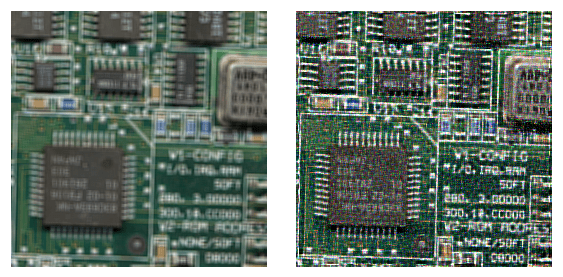
\includegraphics[width=1\textwidth]{img/revisao_bibliografica/desembacamento.png}
    \fonte{Adaptado de \citeonline{mathworks2025lucyrichardson}.}
\end{figure}

\subsection{Detecção de Bordas}
A detecção de bordas identifica limites e formas nas imagens, sendo uma etapa fundamental em muitas tarefas de visão computacional. Redes neurais, como redes de codificação-decodificação, foram desenvolvidas para detectar bordas com alta precisão, superando detectores tradicionais como Canny em imagens ruidosas \cite{yu1994edge}. Métodos inspirados em mecanismos biológicos, como redes com atenção seletiva, melhoraram a extração de características globais, resultando em mapas de bordas mais robustos \cite{chen2022edge}. Essas abordagens são essenciais para pré-processar imagens, fornecendo informações estruturais que facilitam a segmentação e o reconhecimento de objetos \cite{yu1994edge}.

A Figura \ref{fig:deteccao_de_bordas} ilustra o processo de detecção de bordas, onde as bordas da imagem original (à esquerda) são destacadas na imagem processada (à direita).

\begin{figure}[H]
    \centering
    \caption{\label{fig:deteccao_de_bordas}Detecção de Bordas}
    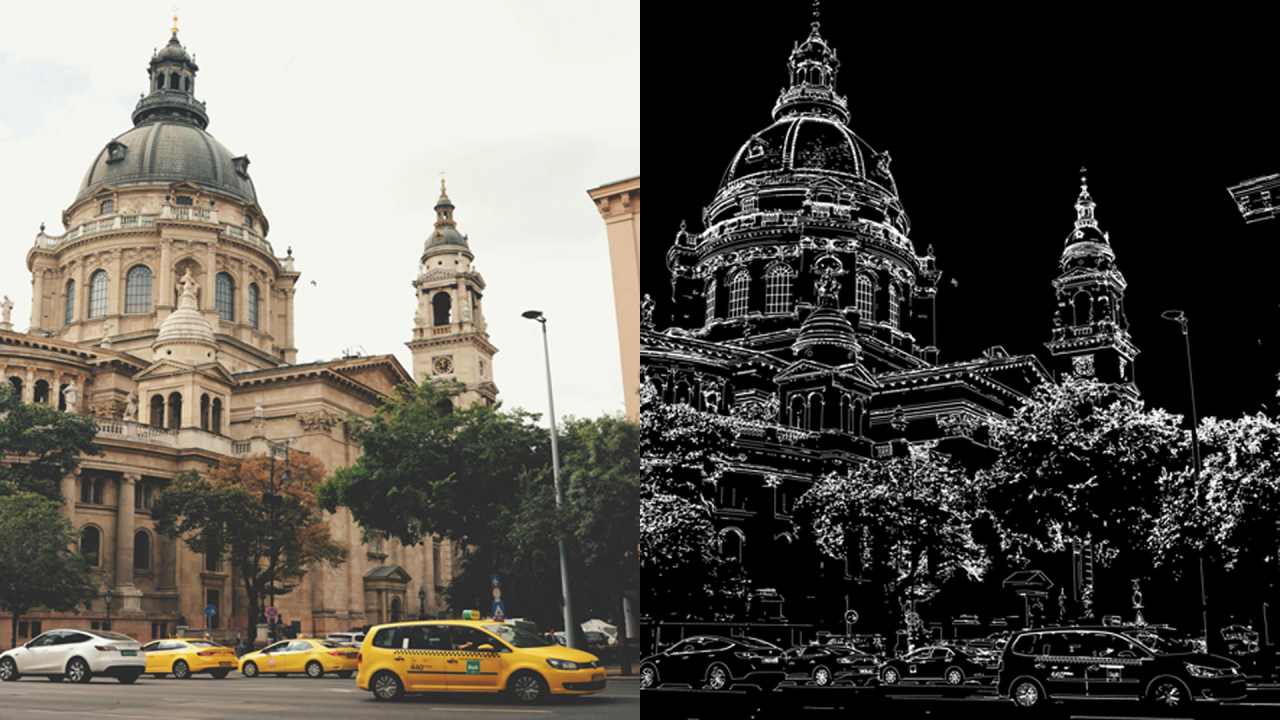
\includegraphics[width=1\textwidth]{img/revisao_bibliografica/deteccao_de_bordas.png}
    \fonte{\citeonline{couto2024regions}.}
\end{figure}

\subsection{Correção de Iluminação}
A correção de iluminação normaliza as condições de luz nas imagens, garantindo consistência na extração de características. Métodos baseados em aprendizado profundo, como redes convolucionais, foram propostos para corrigir imagens com iluminação desigual, como pinturas, alcançando resultados superiores em métricas como NIQE e LOE \cite{li2020simple}. Técnicas híbridas que combinam modelos baseados em aprendizado e físicos foram aplicadas para melhorar a detecção de objetos em condições de luz variada, como em imagens de plantações \cite{yang2022using}. Essas abordagens são particularmente úteis em cenários onde a iluminação não uniforme pode comprometer o desempenho do modelo \cite{li2020simple}.

A Figura \ref{fig:correcao_de_iluminacao} ilustra o processo de correção de iluminação, onde a imagem original (à esquerda) é processada para uniformizar a iluminação, resultando em uma imagem mais equilibrada (à direita).

\begin{figure}[H]
    \centering
    \caption{\label{fig:correcao_de_iluminacao}Correção de Iluminação}
    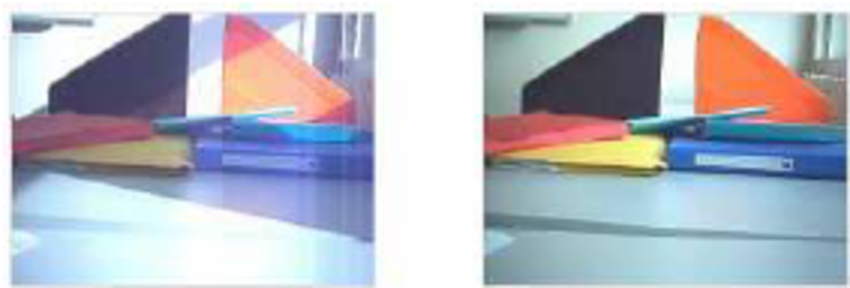
\includegraphics[width=1\textwidth]{img/revisao_bibliografica/correcao_de_iluminacao.png}
    \fonte{\citeonline{Bascle2006IlluminationCorrection}.}
\end{figure}

\subsection{Super-Resolução}
A super-resolução aumenta a resolução de imagens, gerando versões de alta qualidade a partir de entradas de baixa resolução. Redes neurais, como redes convolucionais profundas e redes adversárias generativas (GANs), alcançaram resultados impressionantes, com modelos como SRGAN produzindo imagens fotorrealistas \cite{ledig2017photo}. Em aplicações biológicas, redes como DPA-TISR foram desenvolvidas para imagens de células vivas, alcançando fidelidade temporal e consistência em mais de 10.000 pontos temporais \cite{liu2025neural}. Essas técnicas são valiosas para tarefas que requerem detalhes finos, como análise médica e vigilância, permitindo que redes neurais processem imagens com maior clareza \cite{ledig2017photo}.

\subsection{Conclusão parcial da seção}

O processamento de imagens é uma etapa crucial para garantir a eficácia dos modelos de aprendizado profundo aplicados ao Sistema Elétrico de Potência (SEP). As técnicas discutidas, como normalização, redimensionamento, aumento de dados e redução de ruído, podem ser fundamentais para preparar as imagens antes de serem alimentadas em redes neurais. Essas abordagens não apenas melhoram a qualidade das imagens, mas também garantem que os modelos sejam mais robustos e capazes de generalizar em diferentes condições. A escolha adequada dessas técnicas pode impactar significativamente o desempenho dos modelos na detecção e classificação de falhas em equipamentos de linhas de transmissão.

Dando continuidade, para que as técnicas de processamento de imagens sejam efetivamente aplicadas, é fundamental compreender os fundamentos das redes neurais, que são as principais ferramentas para análise e classificação dessas imagens. A próxima seção aborda os conceitos essenciais sobre redes neurais.

\section{Redes Neurais}
Uma rede neural artificial é formada por um grande número de neurônios para funcionar corretamente, mas para compreender o funcionamento de uma rede neural, deve-se definir o modelo de um único neurônio artificial. Esse modelo é apresentado na Figura~\ref{fig:neuronio}.

\begin{figure}[H]
    \centering
    \caption{\label{fig:neuronio}Modelo de um Neurônio Artificial}
    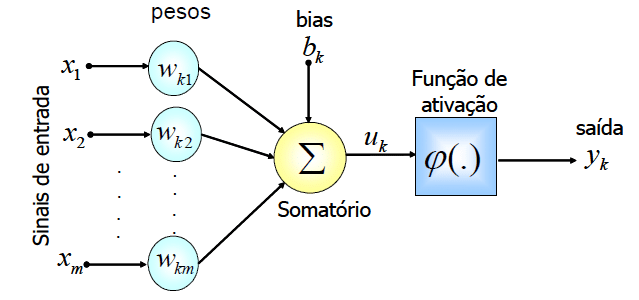
\includegraphics[width=0.8\textwidth]{img/revisao_bibliografica/neuronio.png}
    \fonte{\citeonline{braga2011redes}.}
\end{figure}

Os passos para a obtenção da saída de um neurônio artificial são:

\begin{enumerate}
    \item O modelo recebe um número $m$ de entradas $x_1, x_2, ..., x_m$;
    \item Cada uma dessas entradas é multiplicada por um peso, conforme a Equação~\ref{eq:entrada_peso}:
    \begin{equation}
        x_i w_i, \quad \text{para } i = 1, 2, ..., m
        \label{eq:entrada_peso}
    \end{equation}
    \item Somam-se as entradas multiplicadas pelos seus respectivos pesos, conforme a Equação~\ref{eq:soma_pesos}:
    \begin{equation}
        \sum_{n=1}^{m} w_n x_n
        \label{eq:soma_pesos}
    \end{equation}
    \item Adiciona-se o bias, conforme a Equação~\ref{eq:bias}:
    \begin{equation}
        b + \sum_{n=1}^{m} w_n x_n
        \label{eq:bias}
    \end{equation}
    \item O resultado passa por uma função de ativação, conforme a Equação~\ref{eq:ativacao}:
    \begin{equation}
        \varphi \left( b + \sum_{n=1}^{m} w_n x_n \right)
        \label{eq:ativacao}
    \end{equation}
\end{enumerate}

Seguidos os passos, a equação de saída de um neurônio artificial é descrita pela Equação~\ref{eq:neuronio}.

\begin{equation}
    y = \varphi \left( b + \sum_{n=1}^{m} w_n x_n \right)
    \label{eq:neuronio}
\end{equation}

Visto o modelo de um único neurônio artificial, o conceito de rede neural composta pela associação de diversos neurônios é descrito a seguir.

\subsection{Tipos de redes neurais}

Existem diversos tipos de redes neurais que se distinguem tanto em termos de seus princípios de funcionamento quanto em suas aplicações práticas específicas. A seguir, serão discutidos alguns desses tipos de redes neurais de maneira individualizada, a fim de fornecer uma compreensão mais aprofundada sobre seu funcionamento e suas aplicações \cite{alex2020}.

\subsubsection{Perceptron (P), Feed Forward Network (FFN)}

FFNs são o tipo mais básico de rede neural, em que a informação flui linearmente até a saída e cada neurônio realiza uma operação matemática linear do tipo apresentado na Equação~\ref{eq:wx_b}. Sendo $x$ o valor de entrada, $w$ o peso e $b$ o bias do neurônio. O resultado passa por uma função de ativação e em seguida é enviado para a próxima camada. As redes neurais do tipo FFN (exemplo mostrado através da Figura \ref{fig:ffn}) possuem conexões em apenas um único sentido, geralmente limitadas a 5 camadas \cite{alex2020}.

\begin{equation}
    wx + b
    \label{eq:wx_b}
\end{equation}

\begin{figure}[H]
    \centering
    \caption{\label{fig:ffn}FFN}
    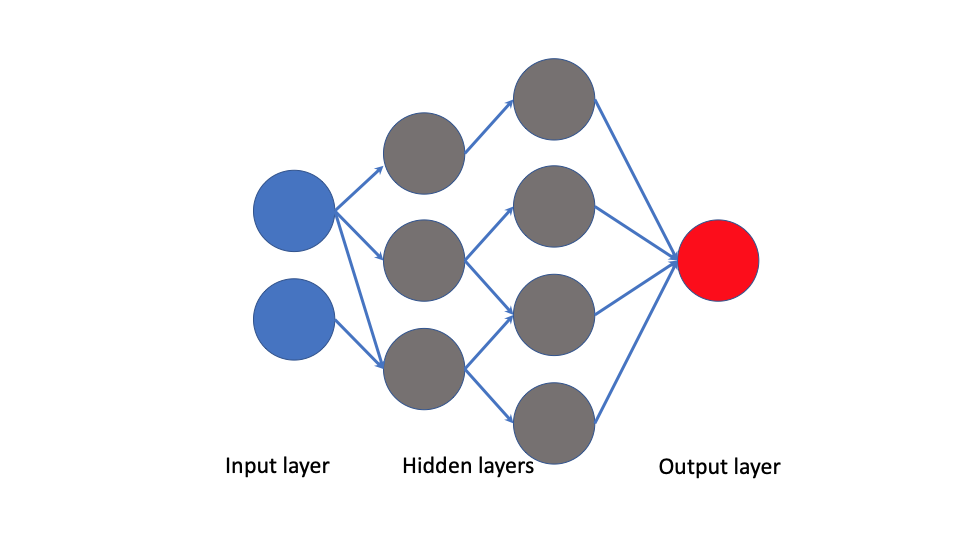
\includegraphics[width=0.8\textwidth]{img/revisao_bibliografica/ffn.png}
    \fonte{\citeonline{alex2020}.}
\end{figure}

As redes do tipo P, Figura \ref{fig:perceptron}, são um caso especial de uma rede FFN, em que todos os neurônios de uma camada são conectados com todos neurônios da camada seguinte \cite{alex2020}.

\begin{figure}[H]
    \centering
    \caption{\label{fig:perceptron}Perceptron}
    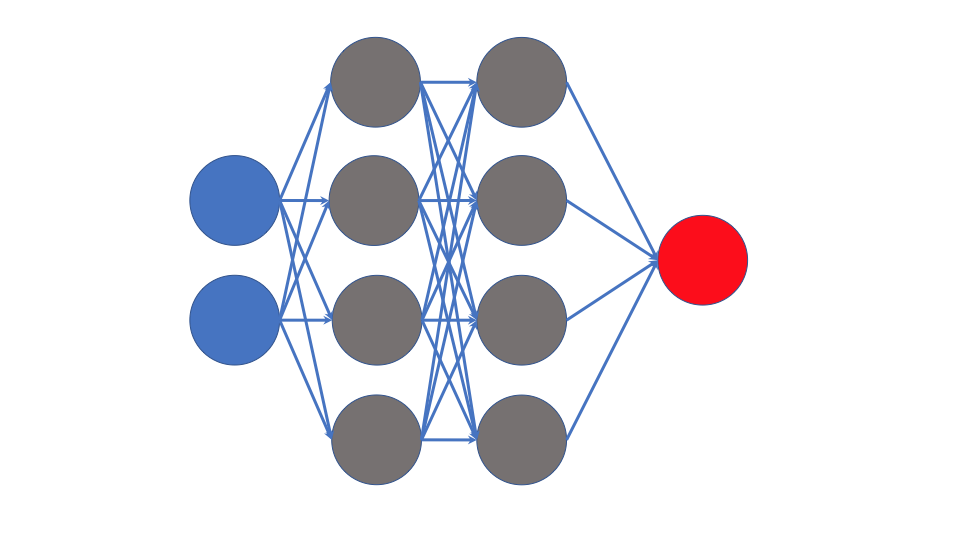
\includegraphics[width=0.8\textwidth]{img/revisao_bibliografica/perceptron.png}
    \fonte{\citeonline{alex2020}.}
\end{figure}

As FFNs são utilizadas para problemas em que os dados de entrada têm impacto atemporal nos dados de saída, em que a saída não depende do estado anterior da rede neural. Um exemplo é usar informações de um exame de sangue para determinar a presença de uma doença.

\subsubsection{Convolutional neural network (CNN) ou Deep convolutional network (DCN)}

As redes neurais estudadas até então, não consideram uma relação de vizinhança entre os dados de entrada. Por exemplo, não faria a menor diferença se antes do treinamento a posição de todos os dados de entrada fossem embaralhadas da mesma forma. Porém, essa relação de vizinhança pode ser muito importante para alguns casos específicos como no reconhecimento de imagens, reconhecimento de voz, análise grafista do mercado financeiro, etc. No reconhecimento de imagens, por exemplo, grande parte da informação está contida na relação de vizinhança dos pixels como o contraste e a textura.

Uma CNN, cuja estrutura está representada através da Figura \ref{fig:cnn}, percebe uma imagem como uma caixa retangular cuja largura e altura são medidas pelo número de pixels da imagem e a profundidade é representada por cada uma das três camadas de cores, vermelho, verde e azul referidas como canais \cite{veen2016}.

\begin{figure}[H]
    \centering
    \caption{\label{fig:cnn}CNN}
    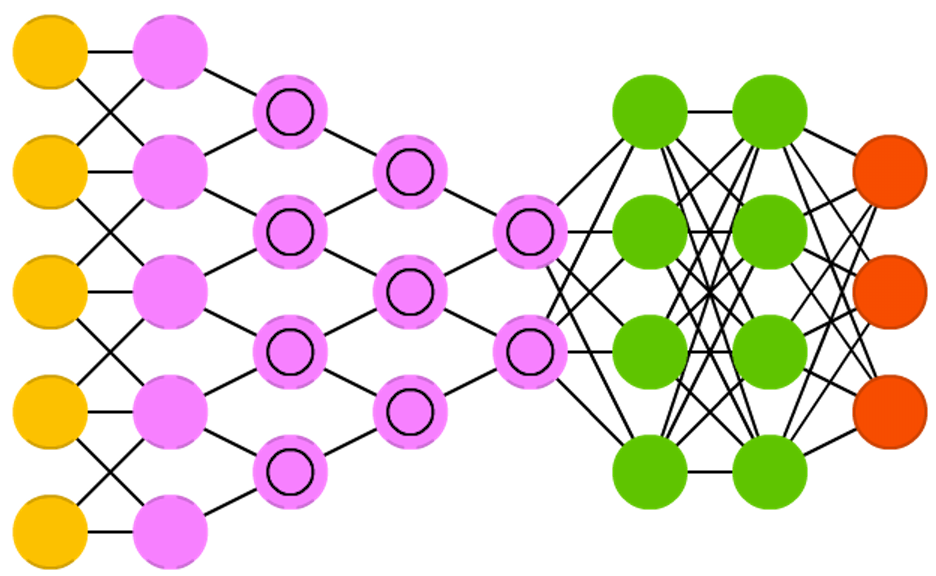
\includegraphics[width=0.8\textwidth]{img/revisao_bibliografica/cnn.png}
    \fonte{\citeonline{veen2016}.}
\end{figure}

Ao longo das camadas de uma rede CNN, as dimensões da imagem se alteram, pois a medida em que a altura e largura da imagem diminuem, o número de canais aumenta, reduzindo o volume de dados. Esse processo é chamado de pooling, que faz um resumo dos dados através do descarte das saídas menos significativas, mantendo somente às de maior valor \cite{veen2016}.

O processo de convolução é realizado arrastando uma janela (kernel) de dimensão menor pela imagem original, sendo essa janela uma rede FFN \cite{veen2016}. Por exemplo, se uma imagem 5x5 pixels passar pelo processo da convolução e supondo uma janela de 3x3 com passo 1 (stride), primeiramente os 3x3 pixels do canto superior esquerdo da imagem original passarão por uma FFN. Em seguida, essa janela é arrastada 1 pixel (tamanho do passo) para a direita e o processo se repete até ao final da imagem.

\subsection{Funções de ativação}

As funções de ativação introduzem não-linearidade nas redes neurais, permitindo que elas aprendam relações complexas entre entradas e saídas. Sem essas funções, mesmo com múltiplas camadas, a rede se comportaria como um modelo linear \cite{badiger2022retrospective}. Cada camada da rede pode ter uma função de ativação diferente, sendo algumas mais adequadas para camadas ocultas e outras para a camada de saída.

A seguir, são apresentadas as três principais funções de ativação:

\subsubsection{ReLU (Rectified Linear Unit)}
Representada pela Equação~\ref{eq:relu}, a ReLU é amplamente utilizada em camadas ocultas. Sua principal vantagem é a eficiência computacional e a aceleração da convergência do gradiente. Contudo, pode causar o problema dos neurônios mortos (Dying ReLU), quando valores negativos resultam sempre em zero \cite{agarap2018deep}.

\begin{equation}
    f(x) = \max(0, x)
    \label{eq:relu}
\end{equation}

\subsubsection{Sigmoid}

Definida pela Equação~\ref{eq:sigmoid}, transforma a entrada em um valor entre 0 e 1, sendo útil para problemas de classificação binária. Apesar de ser diferenciável e fornecer gradientes suaves, sofre com o problema do gradiente pequeno para valores extremos, o que dificulta o aprendizado \cite{langer2020approximating}.

\begin{equation}
    f(x) = \frac{1}{1 + e^{-x}}
    \label{eq:sigmoid}
\end{equation}

\subsubsection{Softmax}
A função Softmax é apresentada na Equação~\ref{eq:softmax} e é utilizada na camada de saída para classificação multiclasse. Ela converte os valores em uma distribuição de probabilidades, acentuando a classe de maior valor \cite{gao2017properties}.


\begin{equation}
    f(x_i) = \frac{e^{x_i}}{\sum_j e^{x_j}}
    \label{eq:softmax}
\end{equation}

\subsubsection{Regras gerais para escolha de funções de ativação}

A escolha da função de ativação depende do tipo de problema e da arquitetura da rede. A seguir, são apresentadas algumas diretrizes gerais:

\begin{itemize}
    \item \textit{Camada de saída:}
    \begin{itemize}
        \item Regressão: Linear
        \item Classificação binária: Sigmoid
        \item Classificação multiclasse: Softmax
        \item Classificação multirrótulo: Sigmoid
    \end{itemize}
    \item \textit{Camadas ocultas:}
    \begin{itemize}
        \item Redes convolucionais: ReLU
        \item Redes recorrentes: Tanh ou Sigmoid
    \end{itemize}
\end{itemize}

\subsection{Funções de Custo}

As funções de custo são responsáveis por medir o quão distante a saída prevista está da saída real. Elas orientam o processo de treinamento ajustando os pesos da rede para minimizar esse erro \cite{rashid2020survey}.

\subsubsection{Erro Médio Quadrático (MSE)}

O Erro Médio Quadrático (MSE) é uma das funções mais comuns em regressão, penalizando fortemente grandes erros e sendo sensível a outliers \cite{chicco2021advantages}. Ele é definido como a Equação~\ref{eq:mse}:

\begin{equation}
    MSE = \frac{1}{n} \sum_{i=1}^{n} (y_i - \hat{y}_i)^2
    \label{eq:mse}
\end{equation}

\subsubsection{Erro Médio Absoluto (MAE)}

O Erro Médio Absoluto (MAE) é mais robusto a outliers que o MSE, mas pode ser mais difícil de otimizar. Sua fórmula é apresentada na Equação~\ref{eq:mae}:

\begin{equation}
    MAE = \frac{1}{n} \sum_{i=1}^{n} |y_i - \hat{y}_i|
    \label{eq:mae}
\end{equation}

\subsubsection{Função Huber}

A função Huber combina as vantagens do MSE e MAE, sendo menos sensível a outliers e mais estável para pequenos erros \cite{huber1964robust}. Ela é definida pela Equação~\ref{eq:huber}:

\begin{equation}
    L_{\text{Huber}} =
    \begin{cases}
        \frac{1}{2}(y - \hat{y})^2 & \text{se } |y - \hat{y}| \leq \delta \\
        \delta (|y - \hat{y}| - \frac{1}{2} \delta) & \text{caso contrário}
    \end{cases}
    \label{eq:huber}
\end{equation}

\subsubsection{Entropia Cruzada Binária}

A Entropia Cruzada Binária é indicada para problemas de classificação binária \cite{zhang2018cross}, sendo expressa pela Equação~\ref{eq:binary_crossentropy}:

\begin{equation}
    L = -\frac{1}{n} \sum_{i=1}^{n} \left[y_i \log(\hat{y}_i) + (1 - y_i) \log(1 - \hat{y}_i)\right]
    \label{eq:binary_crossentropy}
\end{equation}

\subsubsection{Entropia Cruzada Categórica}

Já a Entropia Cruzada Categórica é utilizada em classificação multiclasse com rótulo único por amostra, e sua fórmula é apresentada na Equação~\ref{eq:categorical_crossentropy}:

\begin{equation}
    L = -\sum_{i=1}^{n} \sum_{j=1}^{k} y_{ij} \log(\hat{y}_{ij})
    \label{eq:categorical_crossentropy}
\end{equation}

\subsection{Otimizadores}

Otimizadores são algoritmos que ajustam os pesos da rede neural com base no gradiente da função de custo. Eles influenciam diretamente a velocidade e a qualidade da convergência \cite{ruder2016overview}. Entre os principais otimizadores, destaca-se o Gradiente Descendente, que é a forma mais simples de otimização, mas pode ser lenta e sensível à escolha da taxa de aprendizado. O Gradiente Descendente Estocástico (SGD) atualiza os pesos a cada amostra, adicionando ruído estocástico que pode ajudar a escapar de mínimos locais. O Momentum acrescenta uma fração do gradiente anterior ao atual, acelerando a convergência e suavizando oscilações. O RMSProp ajusta a taxa de aprendizado para cada parâmetro com base na média móvel dos gradientes quadrados \cite{tieleman2012lecture}. Por fim, o Adam combina Momentum e RMSProp, sendo amplamente utilizado por sua eficiência e robustez \cite{kingma2014adam}.

Compreendidos os principais conceitos sobre redes neurais, é importante discutir o papel dos conjuntos de dados (datasets), que são essenciais para o treinamento e avaliação desses modelos. A próxima seção aborda os desafios e técnicas relacionados aos datasets utilizados em tarefas de detecção de falhas.

\section{Datasets}

% Definindo datasets e sua importância
Os conjuntos de dados são fundamentais para o treinamento de redes neurais, fornecendo as amostras necessárias para aprender padrões complexos e realizar previsões precisas. A qualidade, quantidade e diversidade dos dados impactam diretamente o desempenho dos modelos, especialmente em aprendizagem profunda, onde redes com milhões de parâmetros requerem grandes volumes de dados anotados. Conjuntos como o ImageNet, com mais de 14 milhões de imagens em milhares de categorias, foram essenciais para avanços em visão computacional, como a classificação de imagens e detecção de objetos \cite{deng2009imagenet}. Na engenharia elétrica, especificamente na detecção de falhas em cadeias de isoladores e equipamentos de linhas de transmissão, datasets são frequentemente escassos ou desbalanceados, limitando a capacidade dos modelos de generalizar \cite{shorten2019survey}.

% Datasets desbalanceados: definição e desafios
Conjuntos de dados desbalanceados são prevalentes na detecção de falhas em linhas de transmissão, onde amostras de isoladores saudáveis superam significativamente as de defeitos, como quebras ou flashovers (descarga elétrica que ocorre sobre a superfície isolante, quando a rigidez dielétrica é rompida) por poluição. Esse desbalanceamento pode levar a modelos enviesados que favorecem a classe majoritária, resultando em baixa sensibilidade para a detecção de falhas \cite{he2009learning}. Por exemplo, no conjunto de dados IDID, a proporção de isoladores saudáveis para defeituosos é de aproximadamente 10:1 para quebras e 5:1 para flashovers, o que dificulta a classificação precisa das classes minoritárias \cite{oberweger2024xai}. Esse desafio é crítico em aplicações de engenharia elétrica, onde a detecção de falhas raras é essencial para garantir a segurança e a confiabilidade do sistema.

% Datasets escassos: definição e desafios
Datasets escassos, caracterizados por um número reduzido de amostras, são comuns em áreas onde a coleta de dados é custosa, demorada ou restrita pela raridade de eventos, como na detecção de falhas em isoladores de linhas de transmissão. A escassez de dados aumenta o risco de sobreajuste, onde modelos de redes neurais memorizam os dados de treinamento em vez de aprender padrões generalizáveis \cite{goodfellow2016deep}. Esse problema é agravado em aplicações de engenharia elétrica, onde imagens de falhas, como quebras ou flashovers por poluição, são difíceis de obter em quantidade suficiente. A anotação manual de imagens capturadas por drones, frequentemente usada para identificar defeitos, é demorada e propensa a erros, limitando ainda mais o tamanho dos datasets \cite{zheng2022improved}. Por exemplo, o conjunto de dados Insulator-Defect Detection, com apenas 1600 imagens, enfrenta desafios devido ao número limitado de amostras de defeitos \cite{zheng2022improved}.

% Aprendizado por transferência para datasets escassos
O aprendizado por transferência é uma técnica amplamente utilizada para mitigar os desafios de datasets escassos, permitindo que modelos pré-treinados em grandes conjuntos de dados, como o ImageNet, sejam ajustados para tarefas específicas com menos dados \cite{pan2010survey}. Essa abordagem é eficaz em cenários onde características visuais gerais, como bordas e texturas, podem ser transferidas de datasets genéricos para aplicações especializadas. O aprendizado por transferência tem se mostrado particularmente útil em aplicações de engenharia elétrica, onde datasets específicos são frequentemente escassos.

% Aumento de dados para datasets escassos
Uma das formas de tentar diminuir o impacto negativo de bancos de dados escassos, como são os casos citados, é o aumento de dados, uma estratégia essencial para ampliar artificialmente o tamanho e a diversidade dos dados por meio de transformações como rotação, escala, inversão e alterações de iluminação \cite{shorten2019survey}. Esta abordagem é particularmente valiosa quando a coleta de dados reais é custosa, demorada ou limitada pela raridade de eventos, como na detecção de falhas em equipamentos de linhas de transmissão. Na detecção de falhas em linhas de transmissão, essas transformações ajudam a simular diferentes condições ambientais, como variações de luz ou ângulos de captura, comuns em imagens de VANTs (Veículo Aéreo Não Tripulado). Por exemplo, \citeonline{peng2023edf} aplicaram aumento de dados para melhorar a robustez de um modelo YOLOv5 na detecção de defeitos pequenos, como flashovers por poluição, em imagens de linhas de transmissão. Métodos avançados, como redes adversárias generativas (GANs), podem gerar imagens sintéticas de falhas, mas sua aplicação em engenharia elétrica é limitada devido à complexidade computacional \cite{goodfellow2014generative}. Apesar disso, GANs têm potencial para criar amostras sintéticas de defeitos raros, como quebras em isoladores, ampliando datasets escassos e reduzindo significativamente o problema da escassez de dados.

% Aprendizado semi-supervisionado para datasets escassos
O aprendizado semi-supervisionado é uma abordagem promissora para datasets escassos, aproveitando dados não rotulados, que são mais abundantes em inspeções de linhas de transmissão, para melhorar o desempenho do modelo \cite{van2020survey}. Imagens de VANTs capturadas durante inspeções rotineiras podem ser usadas para aprender representações gerais, mesmo sem anotações detalhadas. Embora não haja exemplos específicos na literatura revisada aplicando aprendizado semi-supervisionado diretamente à detecção de falhas em isoladores, \citeonline{chen2020simple} demonstraram sua eficácia em tarefas de visão computacional, sugerindo potencial para aplicações futuras em engenharia elétrica, onde dados não rotulados de inspeções são comuns. Essa técnica pode ser explorada para pré-treinar modelos em grandes conjuntos de imagens de linhas de transmissão antes de ajustá-los em datasets rotulados menores.

% Reamostragem para datasets desbalanceados
A reamostragem é uma técnica comum para abordar o desbalanceamento, envolvendo sobreamostragem da classe minoritária ou subamostragem da classe majoritária para equilibrar a distribuição \cite{johnson2019survey}. Métodos como o SMOTE (Synthetic Minority Over-sampling Technique) geram amostras sintéticas da classe minoritária interpolando exemplos existentes \cite{chawla2002smote}. Em \citeonline{oberweger2024xai}, os autores aplicaram subamostragem para criar partições balanceadas do conjunto de dados IDID, retrainando a última camada do modelo com regressão logística para melhorar a classificação de isoladores defeituosos. Essa abordagem aumentou a precisão em até 12\% para quebras e 7\% para flashovers, demonstrando eficácia em cenários desbalanceados. A reamostragem é particularmente útil quando o número de amostras de defeitos é extremamente baixo, como em datasets de inspeção de linhas.

% Perda focal para datasets desbalanceados
A perda focal é uma função de perda especializada que atribui maior peso a exemplos difíceis, frequentemente pertencentes à classe minoritária, reduzindo o impacto de amostras bem classificadas \cite{lin2017focal}. Na detecção de falhas em isoladores, \citeonline{zheng2022improved} utilizaram a perda focal em um modelo YOLOv7 para lidar com o desbalanceamento entre amostras de isoladores e defeitos em imagens de VANTs. A aplicação dessa técnica melhorou a precisão na detecção de defeitos pequenos, como flashovers por poluição, que são menos frequentes. A perda focal é particularmente vantajosa em tarefas de detecção de objetos, onde o fundo da imagem pode dominar a distribuição de classes, como em imagens de linhas de transmissão com fundos complexos.

% Conjuntos de dados unificados
A unificação de datasets públicos, como proposto por \citeonline{felix2020unifying}, oferece uma abordagem valiosa para a pesquisa em detecção de falhas. O repositório combina datasets como o de Tomaszewski et al. e o CPLID, fornecendo imagens e anotações no formato COCO. Essa consolidação facilita o acesso a dados diversificados, embora o desbalanceamento e a escassez permaneçam desafios que requerem técnicas avançadas de pré-processamento e treinamento. A unificação de datasets é particularmente útil para aumentar o número de amostras disponíveis, permitindo treinar modelos mais robustos para detecção de falhas em isoladores \cite{felix2020unifying}.

A Tabela \ref{tab:tecnicas_escassez_desbalanceamento_datasets} resume os principais datasets utilizados na detecção de falhas em isoladores, destacando suas características e desafios.

\begin{table}[H]
\centering
\caption{Técnicas para Lidar com Escassez e Desbalanceamento de Dados}
\label{tab:tecnicas_escassez_desbalanceamento_datasets}
\begin{tabular}{|p{3.5cm}|p{3.5cm}|p{7.5cm}|}
\hline
\textbf{Categoria} & \textbf{Técnica} & \textbf{Descrição} \\
\hline
Escassez & Aprendizado por Transferência & Reutiliza modelos pré-treinados em grandes conjuntos para tarefas com poucos dados \cite{pan2010survey}. \\
\hline
Escassez & Aumento de Dados & Aplica transformações (por exemplo, rotação, escala) para ampliar o conjunto de dados \cite{shorten2019survey}. \\
\hline
Escassez & Aprendizado Semi-Supervisionado & Aproveita dados não rotulados para aprender representações gerais \cite{van2020survey}. \\
\hline
Desbalanceamento & Reamostragem & Sobreamostra a classe minoritária ou subamostra a majoritária \cite{johnson2019survey}. \\
\hline
Desbalanceamento & Perda Focal & Modifica a perda para focar em exemplos difíceis, geralmente da classe minoritária \cite{lin2017focal}. \\
\hline
\end{tabular}
\end{table}

Após a análise das principais estratégias para lidar com escassez e desbalanceamento de dados, é fundamental compreender como avaliar o desempenho dos modelos desenvolvidos. A seguir, são apresentadas as principais métricas de avaliação utilizadas em tarefas de detecção de falhas em linhas de transmissão.

\section{Métricas de Avaliação de Desempenho de Modelos}

Na detecção de falhas em cadeias de isoladores e equipamentos de linhas de transmissão, a escolha das métricas de avaliação é fundamental para garantir a eficácia e confiabilidade dos modelos de redes neurais. Métricas comumente utilizadas incluem acurácia, precisão, recall, F1-score, área sob a curva ROC (AUC-ROC) e, para tarefas de detecção de objetos, a média da precisão média (mAP). A acurácia, definida como a proporção de previsões corretas em relação ao total, pode ser enganosa em datasets desbalanceados, onde a classe de falhas é significativamente menos representada que a classe de isoladores saudáveis. Por exemplo, em um dataset com 95\% de amostras saudáveis, um modelo que sempre prevê "saudável" alcançará alta acurácia, mas falhará em detectar falhas, comprometendo a segurança do sistema \cite{he2009learning}. Em \citeonline{alam2025robust}, os autores reportaram uma acurácia de 99,96\% para um modelo ensemble RF-LSTM Tuned KNN, mas complementaram a avaliação com precisão, recall e F1-score para abordar o desbalanceamento do conjunto de dados, garantindo uma análise mais robusta do desempenho em classes minoritárias.

A Figura~\ref{fig:roc_curve} ilustra uma curva ROC típica, que representa a relação entre a taxa de verdadeiros positivos (sensibilidade) e a taxa de falsos positivos para diferentes limiares de decisão. A área sob a curva (AUC) é uma métrica importante para avaliar a capacidade discriminativa do modelo.

\begin{figure}[H]
    \centering
    \caption{\label{fig:roc_curve}Curva ROC}
    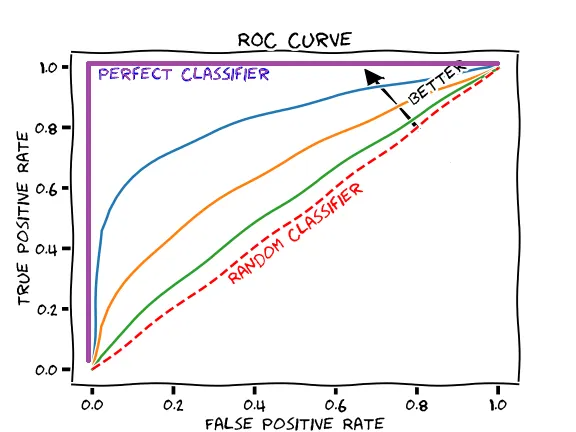
\includegraphics[width=0.7\textwidth]{img/revisao_bibliografica/curva_roc.png}
    \fonte{\citeonline{torres2025}.}
\end{figure}

A precisão mede a proporção de verdadeiros positivos entre todas as previsões positivas, sendo útil para avaliar a confiabilidade das detecções de falhas. O recall, por outro lado, mede a proporção de verdadeiros positivos entre todas as amostras positivas reais, sendo crítico em aplicações onde falsos negativos (falhas não detectadas) podem levar a falhas catastróficas no sistema de transmissão. O F1-score, a média harmônica entre precisão e recall, oferece uma métrica balanceada que considera ambos os aspectos, sendo amplamente utilizado em cenários desbalanceados \cite{johnson2019survey}.

Para tarefas de detecção de objetos, como identificar defeitos em imagens de VANTs, a métrica mAP é padrão, calculando a precisão média para cada classe e tomando a média geral. Em \citeonline{zheng2022improved}, o modelo YOLOv7 foi avaliado no conjunto Insulator-Defect Detection, utilizando mAP para medir a precisão na detecção de quebras e flashovers, com resultados superiores em comparação com modelos anteriores. A AUC-ROC, que avalia a capacidade do modelo de distinguir entre classes em diferentes limiares, também é relevante, especialmente em classificações binárias (falha vs. não falha). Em \citeonline{alam2025robust}, a AUC-ROC foi reportada como 1,0 para classificações binárias, indicando excelente separação entre classes, mas valores menores foram observados em classificações multi-label, refletindo a complexidade de datasets desbalanceados.

Outras métricas, como a matriz de confusão, fornecem uma visão detalhada dos erros do modelo, permitindo calcular taxas de falsos positivos e negativos. Em \citeonline{alam2025robust}, matrizes de confusão foram usadas para avaliar o desempenho do modelo ensemble em classificações binárias e multi-label, complementando as métricas de precisão e recall. Para aplicações em tempo real, como inspeções de VANTs, métricas adicionais, como tempo de inferência e complexidade computacional, também são consideradas, especialmente em modelos como YOLOv5 e YOLOv7, que priorizam eficiência \cite{peng2023edf}. A escolha das métricas deve, portanto, alinhar-se com os objetivos da aplicação, priorizando recall para segurança e mAP para detecção precisa de objetos em imagens.

Por fim, compreender as métricas de avaliação é essencial para interpretar corretamente os resultados obtidos com diferentes modelos e técnicas de processamento de imagens. A próxima etapa do trabalho irá detalhar a metodologia proposta para aprimoramento dos processamentos e avaliação dos modelos.

A Tabela~\ref{tab:metricas_avaliacao_modelos} apresenta um resumo das principais métricas utilizadas para avaliar o desempenho de modelos em tarefas de detecção de falhas em linhas de transmissão, destacando suas características e aplicações.

\begin{table}[H]
\centering
\caption{Principais métricas de avaliação de desempenho de modelos}
\label{tab:metricas_avaliacao_modelos}
\begin{tabular}{|p{4.5cm}|p{10cm}|}
\hline
\textbf{Métrica} & \textbf{Descrição} \\
\hline
Acurácia & Proporção de previsões corretas em relação ao total de amostras. Pode ser enganosa em conjuntos desbalanceados. \\
\hline
Precisão & Proporção de verdadeiros positivos entre todas as previsões positivas. Mede a confiabilidade das detecções. \\
\hline
Recall (Sensibilidade) & Proporção de verdadeiros positivos entre todas as amostras positivas reais. Mede a capacidade de encontrar todos os casos positivos. \\
\hline
F1-score & Média harmônica entre precisão e recall. Útil para avaliar o desempenho em cenários desbalanceados. \\
\hline
mAP (mean Average Precision) & Média das precisões médias para cada classe. Padrão em tarefas de detecção de objetos. \\
\hline
AUC-ROC & Área sob a curva ROC. Mede a capacidade do modelo de distinguir entre classes em diferentes limiares. \\
\hline
Matriz de Confusão & Tabela que mostra as previsões corretas e incorretas, detalhando verdadeiros/falsos positivos e negativos. \\
\hline
\end{tabular}
\end{table}

\section{Considerações finais do capítulo}

Neste capítulo, foram apresentados os principais conceitos e técnicas de processamento de imagens, redes neurais, estratégias para lidar com escassez e desbalanceamento de dados, além das métricas de avaliação de desempenho de modelos aplicados à detecção de falhas em linhas de transmissão. A revisão evidenciou que o uso de métodos avançados de processamento de imagens e aprendizado profundo é fundamental para garantir a confiabilidade e eficiência do Sistema Elétrico de Potência, especialmente em cenários desafiadores, como a inspeção de grandes extensões e a identificação de defeitos raros.

A escolha adequada das técnicas de pré-processamento, arquitetura de redes neurais e estratégias para tratar limitações dos datasets impacta diretamente na robustez e precisão dos modelos desenvolvidos. Além disso, a seleção criteriosa das métricas de avaliação permite uma análise mais completa do desempenho, especialmente em situações de desbalanceamento entre classes.

Portanto, o domínio desses conceitos é essencial para o desenvolvimento de soluções inovadoras e eficazes na área de inspeção automatizada de linhas de transmissão, contribuindo para a segurança, confiabilidade e continuidade do fornecimento de energia elétrica. O próximo capítulo irá detalhar a metodologia proposta para aprimoramento dos processamentos e avaliação dos modelos, consolidando os fundamentos discutidos nesta revisão.
